\documentclass[11pt]{beamer}
\usetheme{Dresden}
\usepackage[utf8]{inputenc}
\usepackage{amsmath}
\usepackage{amsfonts}
\usepackage{amssymb}
\usepackage{graphicx}
\usepackage{verbatim}
\usepackage{listings}
\usepackage{xcolor}

\let\OldTexttt\texttt
\renewcommand{\texttt}[1]{\OldTexttt{\color{teal}{#1}}}

\definecolor{eggplant}{rgb}{0.5, 0.25, 0.5} % UBC Blue (primary)

\usecolortheme[named=eggplant]{structure}


\definecolor{mGreen}{rgb}{0,0.6,0}
\definecolor{mGray}{rgb}{0.5,0.5,0.5}
\definecolor{mPurple}{rgb}{0.58,0,0.05}
\definecolor{mGreen2}{rgb}{0.05,0.65,0.05}
\definecolor{mGray2}{rgb}{0.55,0.55,0.55}
\definecolor{mPurple2}{rgb}{0.63,0.05,0.05}
\definecolor{backgroundColour}{rgb}{0.95,0.95,0.92}
\definecolor{backgroundColour2}{rgb}{0.95,0.92,0.95}

\lstdefinestyle{C}{
    backgroundcolor=\color{backgroundColour},   
    commentstyle=\color{mGreen},
    keywordstyle=\color{blue},
    numberstyle=\tiny\color{mGray},
    stringstyle=\color{mPurple},    
    basicstyle=\footnotesize,
    breakatwhitespace=false,         
    breaklines=true,                 
    captionpos=b,                    
    keepspaces=true,                 
    numbers=left,                    
    numbersep=5pt,                  
    showspaces=false,                
    showstringspaces=false,
    showtabs=false,                  
    tabsize=2,
    language=C
}

\lstdefinestyle{Python}{
    backgroundcolor=\color{backgroundColour2},   
    commentstyle=\color{mGreen2},
    keywordstyle=\color{blue},
    numberstyle=\tiny\color{mGray2},
    stringstyle=\color{mPurple2},
    basicstyle=\footnotesize,
    breakatwhitespace=false,         
    breaklines=true,                 
    captionpos=b,                    
    keepspaces=true,                 
    numbers=left,                    
    numbersep=5pt,                  
    showspaces=false,                
    showstringspaces=false,
    showtabs=false,                  
    tabsize=2,
    language=Python
}

\author{NCC Moore}
\title{Topic 4 - Basic Constructs in C}
%\setbeamercovered{transparent} 
%\setbeamertemplate{navigation symbols}{} 
%\logo{} 
\institute{McMaster University} 
\date{Summer 2021} 
\subject{COMPSCI 1XC3 - Computer Science Practice and Experience:
Development Basics} 
\stepcounter{section}
\begin{document}

\begin{frame}
\center
COMPSCI 1XC3 - Computer Science Practice and Experience:
Development Basics
\titlepage
(Loosely) Adapted from C: How to Program 8th ed., Deitel \& Deitel
\end{frame}

\begin{frame}
\tableofcontents
\end{frame}



\section[Intro]{Getting Started}
\begin{frame}[fragile=singleslide]{A Simple Sample}
\begin{lstlisting}[style=C]
// A REALLY simple program in C
#include <stdio.h>

// the 'main' function begins program execution
int main(void) {
	printf("Hello World!\n");
} // end function main
\end{lstlisting}
\end{frame}

\begin{frame}[fragile=singleslide]{Comment Your Code! (Or Else!)}
\begin{itemize}
\item In Python, \texttt{\#} designates a single-line comment.
\begin{itemize}
\item In C, \texttt{//} is used.
\end{itemize}
\item C also has Multi-line comments! 
\end{itemize}
\begin{lstlisting}[style = C]
/* This is a multi-line comment! 
 * 
 *
 * Yup, still going...
 *
 */
\end{lstlisting}
\begin{itemize}
\item \texttt{\textbf{/*}} begins a multi-line comment.
\item \texttt{\textbf{*/}} ends the comment.  
\end{itemize}
\end{frame}

\begin{frame}{Comment Your Code! (Or Else!) (cont.)}
Here are some guidelines for commenting code in C:
\begin{itemize}
\item At the top of the file, indicate:
	\begin{itemize}
	\item The author
	\item The date the program was created
	\item The date the program was last modified
	\item The purpose of the program
	\end{itemize}
\item Comment each function to indciate what its purpose is.  This includes any assumptions about the inputs, properties of the outputs and invariants that will hold throughout execution.
\item Comment the end of each function with something like ``end of function x''.  This will make it much easier to navigate your code.
\end{itemize}
\end{frame}

\begin{frame}{Preprocessor Directives}
\begin{itemize}
\item In Python, we access libraries using \texttt{import ...}
\item In C, we use \texttt{\#include<...>}
\begin{itemize}
\item Lines beginning with \# are \textbf{preprocessor directives}
\item Preprocessor directives are processed before the program is parsed.  
\item \textbf{*.h} files are known as \textbf{header files}.  Many of C's most important libraries are stored in header files.  
\item \texttt{stdio.h} contains the definition for \texttt{printf} (and much more besides!)  
\item Adding the line \texttt{\#include<stdio.h>} to the beginning of each C program should become reflexive! 
\end{itemize}
\end{itemize}
\end{frame}

\begin{frame}[fragile=singleslide]{Being a Blockhead}
\begin{itemize}
\item In Python, statement blocks are indicated using indentation.
\begin{lstlisting}[style=Python]
def max2(x,y) :
	if (x > y) :
		return x
	else :
		return y
\end{lstlisting}
\item In C, statement blocks are indicated using \texttt{$\{$} and \texttt{$\}$}
\begin{lstlisting}[style=C]
int max2(int x, int y) {
	if (x > y) {
		return x;
	} else {
		return y;
	}
}
\end{lstlisting}
\item In addition, \emph{all C statements are semicolon terminated;}
\end{itemize}
\end{frame}

\begin{frame}[fragile=singleslide]{Whitespace Doesn't Matter!}
This C program...
\begin{lstlisting}[style=C]
#include<stdio.h>

int main (void) { 
	int x = 17;
	bool y = False;
	if (y == False) {
		return x;
	} else {
		return -1;
	}
}
\end{lstlisting}
\end{frame}
\begin{frame}[fragile=singleslide]{Whitespace Doesn't Matter! (cont.)}
Is \emph{identical} to this C program...
\begin{lstlisting}[style=C]
#include<stdio.h>
int main (void) { /* Midline comments! */ int x = 17; bool y 
= False;
	
					if (y ==         False){return x;
} else { return -1;}}
\end{lstlisting}
At least as far as the compiler is concerned! 

(Clearly, one of these is preferrable...)
\end{frame}

\begin{frame}{The \texttt{main} Event}
\begin{itemize}
\item In Python, execution begins at the first line of the script, and terminates on the last line.  
\item In C, execution begins at the first line of the \texttt{main} function(!), and terminates either when execution reaches a \texttt{return} statement inside of \texttt{main}, or when the program reaches the last line of \texttt{main}.
\item A \texttt{main} function is required for compilation
\item Trying to put regular statements in the global namespace will result in \emph{Syntax Errors A'Plenty!}
\end{itemize}
We'll talk about other functions in C in excruciating depth in the next few weeks.
\end{frame}

\begin{frame}[fragile=singleslide]{The \texttt{main} Event (cont.)}
\begin{lstlisting}[style=C]
...
int main (void) { 
	...
}
...
\end{lstlisting}
\begin{itemize}
\item The \texttt{int} keyword indicates that \texttt{main} returns an integer value.
	\begin{itemize}
	\item A return value of 0 indicates the program exited normally (i.e., without runtime errors).
	\item Any other return value typically indicates the program exited abnormally (i.e., errors happened!)
	\end{itemize}
\item Giving \texttt{void} as an argument indicates that this program is ignoring any passed arguments.  The \texttt{void} keyword may be omitted.
\end{itemize}
\end{frame}

\section[I/O]{Simple Input/Output}
\begin{frame}[fragile=singleslide]{\texttt{printf()} and \texttt{stdout}}
Printing strings should be nothing new, but let's go over it anyways.
\begin{itemize}
\item \texttt{printf()} is equivalent to Python's \texttt{print()} function
\begin{itemize}
\item The biggest difference is that \texttt{printf()} does \emph{not} automatically append \texttt{\textbackslash n} to the end of a string.
\end{itemize} 
\end{itemize}
\begin{lstlisting}[style=C]
	printf("From one string ");
	printf("to the next,\nEveryone Lo");
	printf("ves Lisp!");
\end{lstlisting}
Will produce the output:
\hrule
\begin{verbatim}
From one string to the next, 
Everyone Loves Lisp!
\end{verbatim}
\hrule
\end{frame}

\begin{frame}{String Formatting!}
String formatting should also be nothing new, but there are some important differences.
\begin{itemize}
\item In Python, strings are delimited by either double or single quotes (\texttt{"Hello World"} $\equiv$ \texttt{'Hello World'})
\item In C, single and double quotes have different meanings! 
\begin{itemize}
\item Double quotes are \emph{string} delimiters.
\item Single quotes are \emph{character} delimiters.
\end{itemize}
\end{itemize}
\center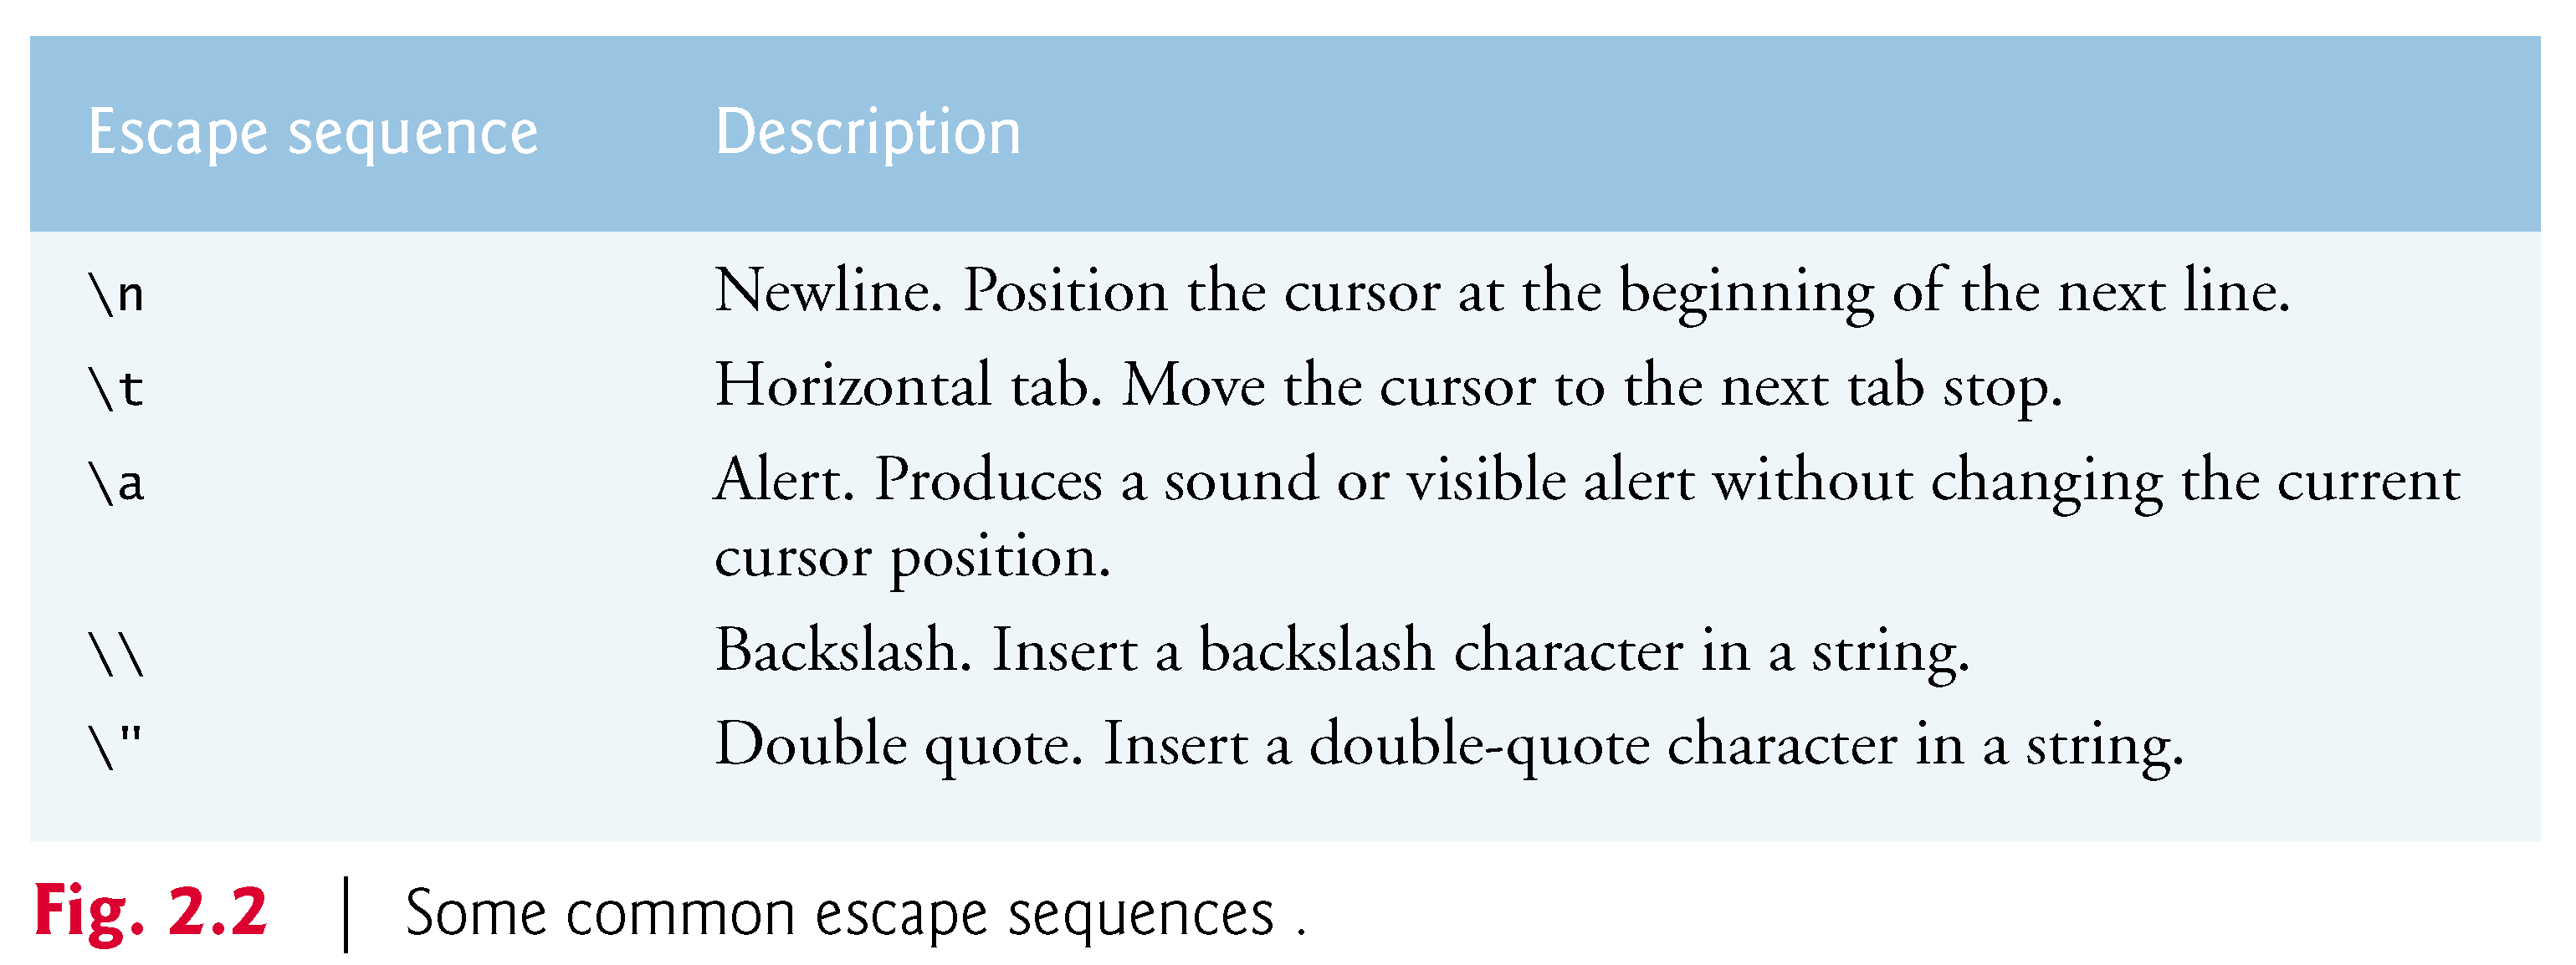
\includegraphics[scale=0.1]{escape.png}
\end{frame}

\begin{frame}[fragile=singleslide]{Reading from \texttt{stdin}}
The following program uses the \texttt{scanf} standard library function to read keystrokes from the \texttt{stdin} buffer.
\begin{lstlisting}[style=C]
// Program to add two numbers with user prompts
#include <stdio.h>

int main (void) { 
	int i1;
	int i2;
	printf("Enter your first integer\n");
	scanf("%d", &i1);
	printf("Enter your second integer\n");
	scanf("%d", &i2);
	printf("The sum is %d\n", (i1 + i2));
} // end of main
\end{lstlisting}
\end{frame}

\begin{frame}[fragile=singleslide]{Reading from \texttt{stdin} (cont.)}
When executed, the following output is produced.  
\hrule
\begin{verbatim}
Enter your first integer
5
Enter your second integer
9
The sum is 14
\end{verbatim}
\hrule
\end{frame}

\begin{frame}[fragile=singleslide]{\texttt{scanf} and \texttt{stdin}}
The standard library function \texttt{scanf} reads characters from the standard input buffer \texttt{stdin}.  
\begin{lstlisting}[style=C]
scanf("%d", &i1);
\end{lstlisting}
\begin{itemize}
\item The first argument is a \textbf{format control string}, which indicates the data type that should be input by the user. (\texttt{\%d} means \texttt{int})
\item The second argument is the variable we want \texttt{scanf} to put the data in, prepended with the \textbf{adress of operator} \texttt{\&}.
\item We will be covering \texttt{\&} in depth when we talk about \textbf{pointers}...
\end{itemize}
\end{frame}

\begin{frame}[fragile=singleslide]{Revisiting \texttt{printf}}
\begin{lstlisting}[style=C]
printf("The sum is %d", (i1 + i2));
\end{lstlisting}
\begin{itemize}
\item To print the value of a variable, you must:
\begin{itemize}
\item use a \textbf{format specifying placeholder} in the first argument
\item supply the variable as the second argument
\end{itemize}
\item Each data type has it's own placeholder.
\end{itemize}
\end{frame}

\begin{frame}[fragile=singleslide]{Declaring Variables}
You may have noticed that the above program uses variables
\begin{itemize}
\item Variables in C work the same as in other C-based languages.
\item In contrast to Python, C variables require explicit declaration.
\item A variable must be declared with a data type (in this case \texttt{int}), like so:
\begin{lstlisting}[style=C]
	int x, y;
	float z;
\end{lstlisting}
\item Variables may also be declared with an initial value:
\begin{lstlisting}[style=C]
	int x = 7, y = 8;
	float z = 3.14;
\end{lstlisting}
\item This is known as \textbf{instantiation}.
\end{itemize}
\end{frame}

\section[Types]{Fundamental Data Types}
\begin{frame}{Fundamental Data Types}
\small \center
\begin{tabular}{| c | c | c | c |}
\hline
Declaration & Size (bytes) & placeholder \\ \hline
\texttt{short int} & 2 & \%hd \\ \hline
\texttt{unsigned short int} & 2 & \%hu \\ \hline
\texttt{unsigned int} & 4 & \%u \\ \hline
\texttt{int} & 4 & \%d \\ \hline
\texttt{long int} & 8 & \%ld \\ \hline
\texttt{unsigned long int} & 8 & \%lu \\ \hline
\texttt{long long int} & 8 & \%lld \\ \hline
\texttt{unsigned long long int} & 8 & \%llu \\ \hline
\texttt{signed char} & 1 & \%c \\ \hline
\texttt{unsigned char} & 1 & \%c \\ \hline
\texttt{float} & 4 & \%f \\ \hline
\texttt{double} & 8 & \%lf \\ \hline
\texttt{long double} & 16 & \%Lf \\ \hline
\end{tabular}
\end{frame}

\begin{frame}[fragile=singleslide]{Don't give me that Bool!}
You may have noticed that the foregoing slide didn't have booleans on it! 
\begin{itemize}
\item Boolean support was added to C in ISO/IEC 9899:1999, which came out in 1999.
\item Unlike most other languages, booleans are not part of the C prelude! In order to use them, you have to include the standard boolean library.
\item Add this line to your set of include statements:
\begin{lstlisting}[style=C]
#include<stdbool.h>
\end{lstlisting}
\item Before this library, C programmers would use \texttt{int}'s to represent boolean values.
\begin{itemize}
\item 0 $\equiv$ False
\item All other values $\equiv$ True (1 is typically used).
\end{itemize}
\end{itemize}
\end{frame}

\section[Memory]{More Memory Concepts}
\begin{frame}{More Memory Concepts}
\begin{itemize}
\item \textbf{Variables} are units of memory that have been assigned an identifier.  
\item The amount of memory allocated is dependent on the data type the variable is declared with.
\item The specific arrangement of 1's and 0's at the memory location the variable indicates is the value of that variable.
\item When a new value is assigned to a variable, the underlying memory is overwritten with the new value (i.e., the process is \emph{destructive}).
\item Reading a variable is \emph{non-destructive}.
\end{itemize}
\end{frame}

\begin{frame}{Static vs Dynamic Typing}
\begin{itemize}
\item In Python, variables don't need to be declared with a data type (\textbf{Dynamic Typing})
\begin{itemize}
	\item The Python interpreter manages the memory representation of variables
\end{itemize}
\item In C, the type declaration tells the memory system how much memory to reserve for the variable, so the information must be present! 
\item This is known as \textbf{Static Typing}.
\item Variables in the same program will not necessarily be allocated adjacent memory cells! 
\end{itemize}
\end{frame}


\section[Operators]{Operator Roundup}
\begin{frame}{Operator? Get me Chicago!}
\center
\begin{tabular}{| c | c |}
\hline
Description & Syntax \\ \hline
Increment (postfix) & \texttt{x ++} \\ \hline
Decrement (postfix) & \texttt{x --} \\ \hline
Increment (prefix) & \texttt{++ x} \\ \hline
Decrement (prefix) & \texttt{-- x} \\ \hline
Negation & \texttt{-x} \\ \hline
Arithmetic Addition & \texttt{x + y} \\ \hline
Arithmetic Subtraction & \texttt{x - y} \\ \hline
Aritmetic Multiplication & \texttt{x * y} \\ \hline
Aritmetic Division & \texttt{x / y} \\ \hline
Aritmetic Modulus & \texttt{x \% y} \\ \hline
\end{tabular}
\end{frame}

\begin{frame}{Incremental Improvement}
\begin{itemize}
\item The increment and decrement operators (\texttt{++} and \texttt{--} respectively) either add or subtract 1 from the operand.  
\item \texttt{++} and \texttt{--} use \textbf{implicit assignment}, so no assignment operator is required!
\item Whether the operator is prefix or postfix effects the semantics  
\begin{itemize}
\item If the operator is prefix (\texttt{++x}), the increment/decrement is executed \emph{before} the containing expression.
\item If the operator is postfix (\texttt{x--}), the increment/decrement is executed \emph{after} the containing expression.
\end{itemize}
\item Because of this implicit assignment, using \texttt{++} or \texttt{--} on an integer literal is a \emph{syntax error}!
\end{itemize}
\end{frame}

\begin{frame}[fragile=singleslide]{Incremental Example}
\begin{lstlisting}[style=C]
#include <stdio.h>
int main() {
   int var1 = 5, var2 = 5;

   // var1 is displayed
   // Then, var1 is increased to 6.
   printf("Variable 1 = %d\n", var1++);

   // var2 is increased to 6 
   // Then, it is displayed.
   printf("Variable 2 = %d\n", ++var2);

   return 0;
}
\end{lstlisting}
\hrule
\begin{verbatim}
Variable 1 = 5
Variable 2 = 6
\end{verbatim}
\end{frame}

\begin{frame}{It's All Relational}
\center
\begin{tabular}{| c | c | c |}
\hline
Relational Operators & Syntax \\ \hline
Equality & \texttt{x == y} \\ \hline
Inequality & \texttt{x != y} \\ \hline
Greater than & \texttt{x > y} \\ \hline
Greater than or equal to & \texttt{x >= y} \\ \hline
Less than & \texttt{x < y} \\ \hline
Less than or equal to & \texttt{x <= y} \\ \hline \hline
Logical Operators & Syntax \\ \hline
Not & \texttt{!x} \\ \hline
And & \texttt{x \&\& y} \\ \hline
Or & \texttt{x \textbar\textbar \hspace{1pt} y} \\ \hline
\end{tabular} 
\end{frame}

\begin{frame}[fragile=singleslide]{For Your Next Assignment...}
\center
\begin{tabular}{| c | c | c |}
\hline
Description & Syntax & Equivalent to \\ \hline
Assignment & \texttt{x = y} & -- \\ \hline
Assignment plus addition & \texttt{x += y} & \texttt{x = x + y} \\ \hline
Assignment plus subtraction & \texttt{x -= y} & \texttt{x = x - y} \\ \hline
Assignment plus multiplication & \texttt{x *= y} & \texttt{x = x * y} \\ \hline
Assignment plus division & \texttt{x /= y} & \texttt{x = x / y} \\ \hline
Assignment plus modulus & \texttt{x \%= y} & \texttt{x = x \% y} \\ \hline
\end{tabular}
\end{frame}

\section[Branching]{Selective Structures}
\begin{frame}[fragile=singleslide]{\texttt{if}fy Subject Matter}
If statements are a bit different in C vs Python.
\begin{lstlisting}[style=C]
	if (<condition>) {
		<statments>
	} else {
		<statements>
	}
\end{lstlisting}
In particular, elif is replaced with:
\begin{lstlisting}[style=C]
	if (<condition1>) {
		<statements>
	} else if (<condition2>) {
		<statements>
	} else {
		<statements>
	}	
\end{lstlisting}
\end{frame}

\begin{frame}
\center
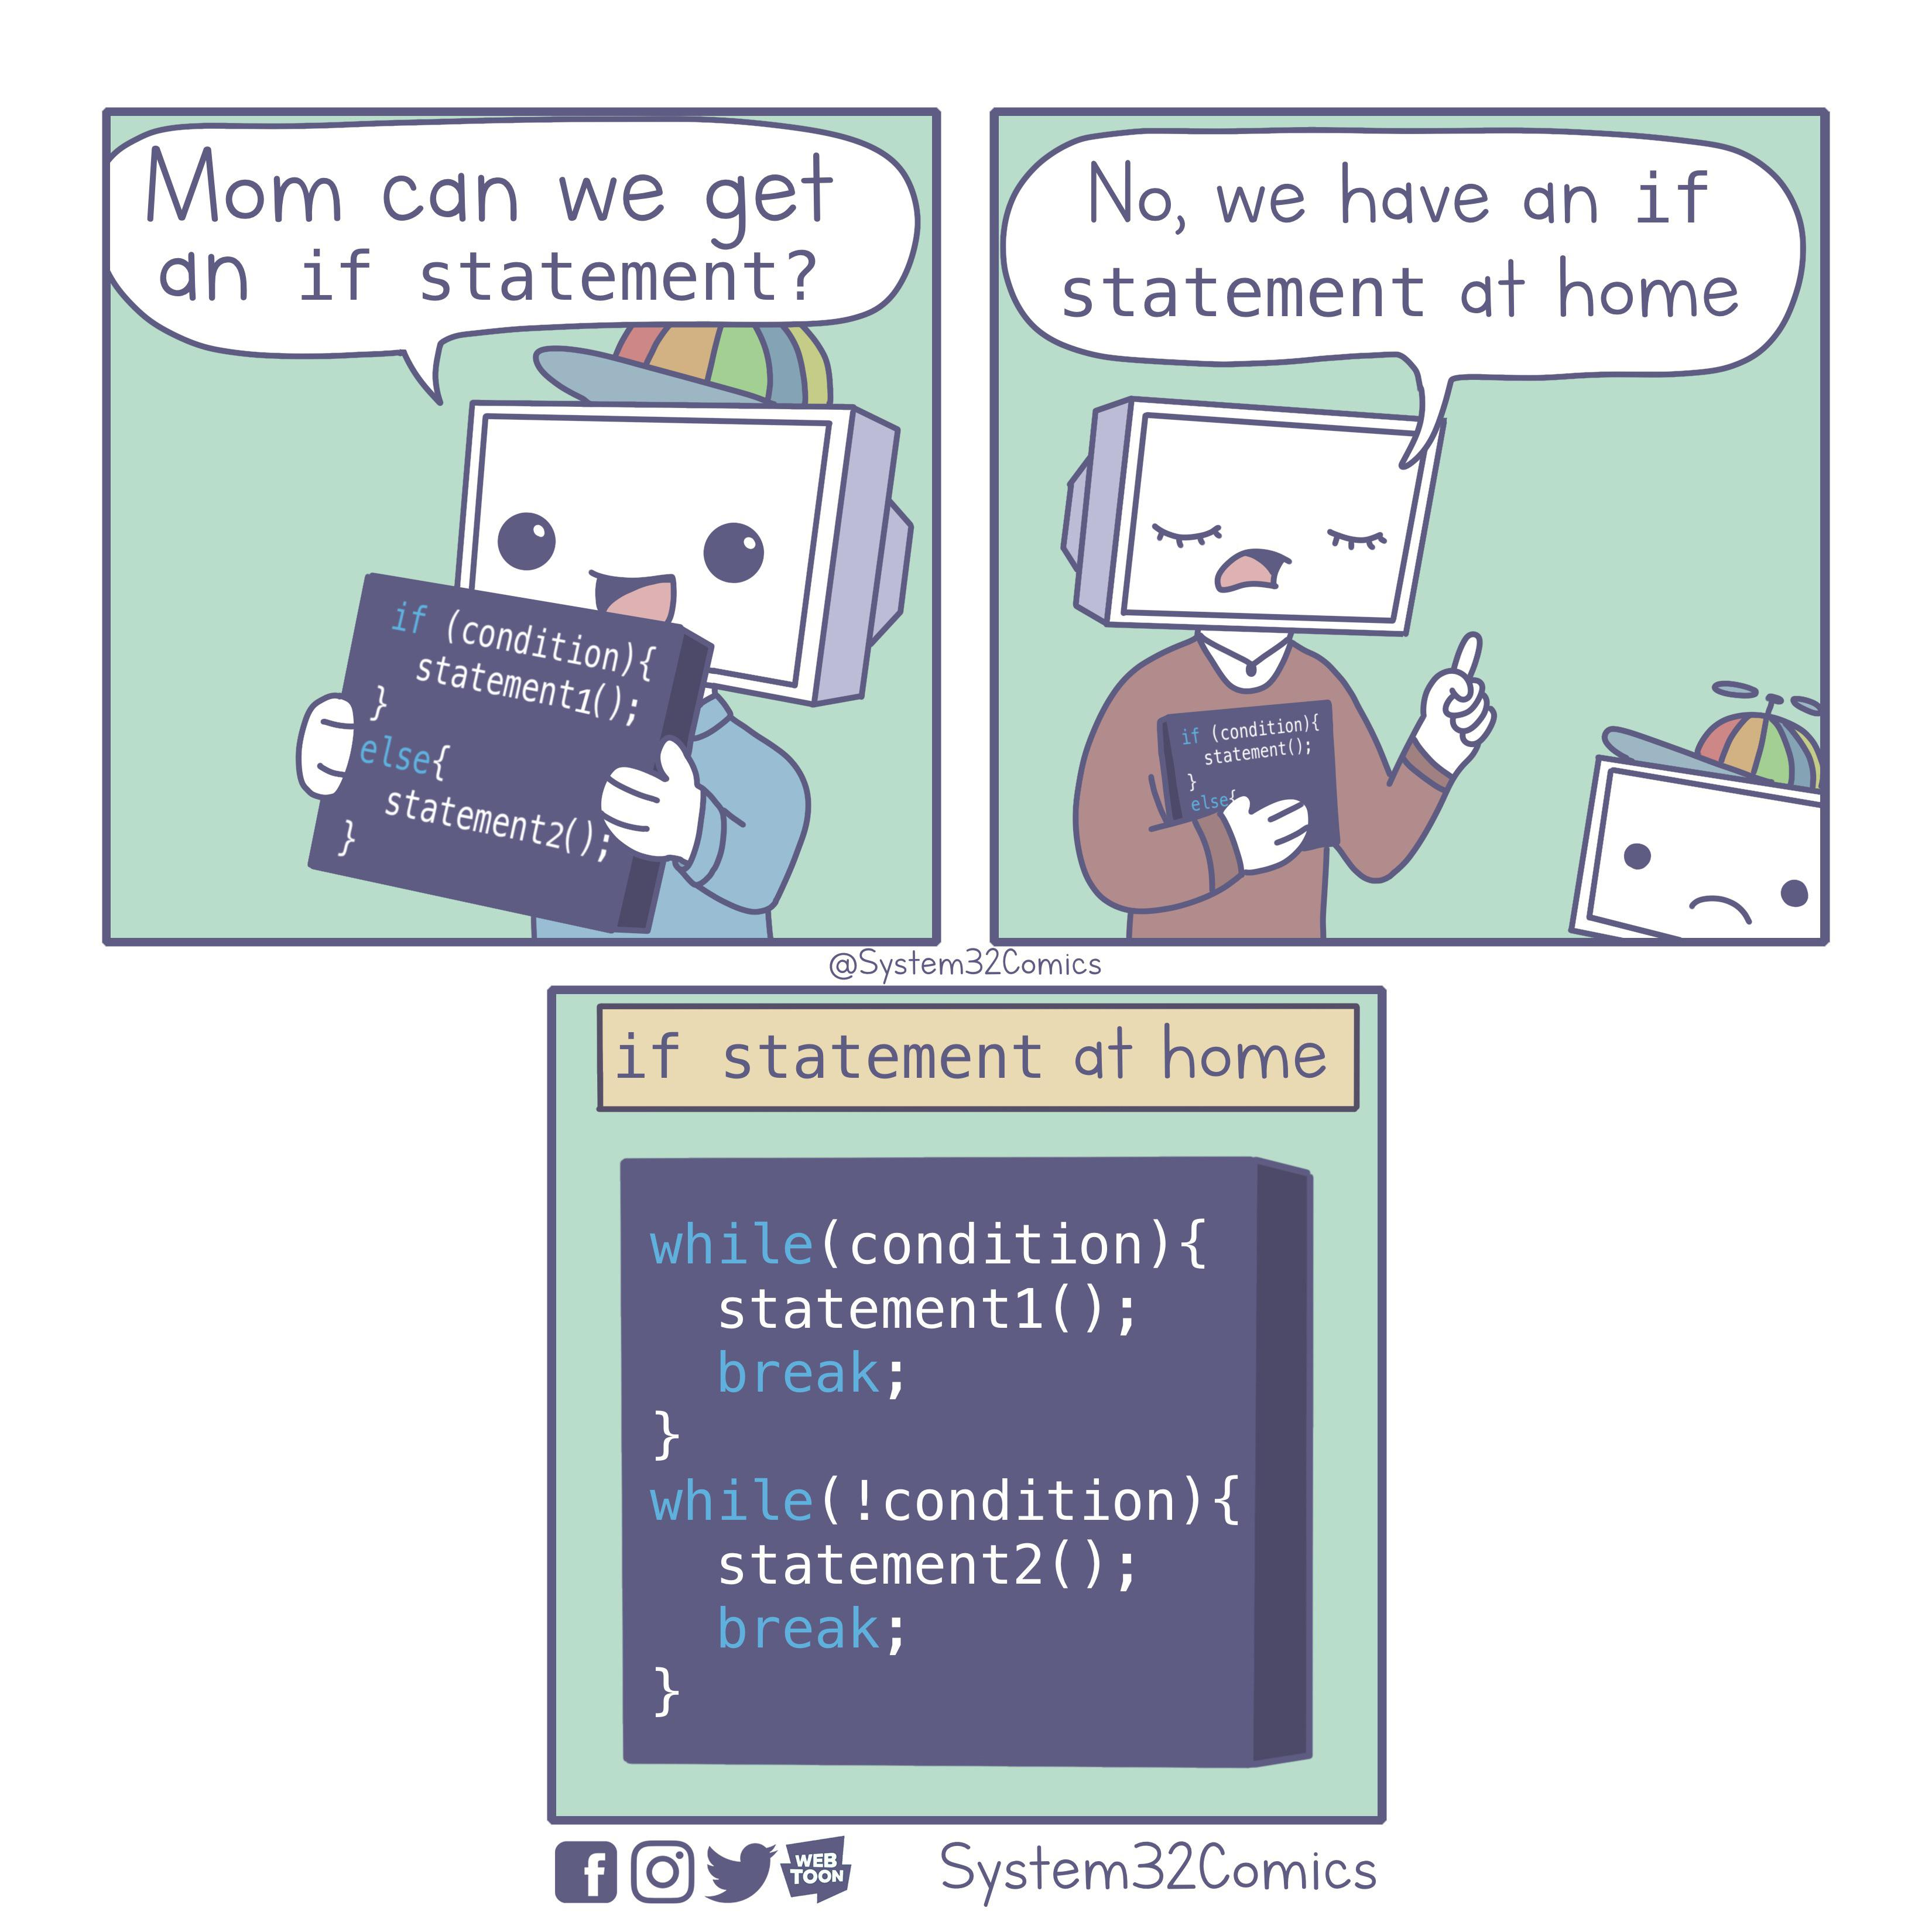
\includegraphics[scale=0.065]{ifstatement.jpg}
\end{frame}

\begin{frame}[fragile=singleslide]{Let's \texttt{switch}, just in \texttt{case}}
Python dropped \texttt{switch} blocks in favour of \texttt{elif}.
\begin{lstlisting}[style=C]
	switch (x) {
		case 1: // executes if x == 1
			break;
		case 2: // executes if x == 2
			// no break means control flows to next case
		case 3: // executes if x == 2 || x == 3
			break;
		default: // executes if x != 1, 2 or 3
	}	
\end{lstlisting}
\end{frame}

\begin{frame}{Let's \texttt{switch}, just in \texttt{case} (cont.)}
\begin{itemize} 
\item In this example, \texttt{x} is the \textbf{controlling expression}.
\item The value of the controlling expression is compared to each \textbf{case label}, which is a literal of the return type of the controlling expression.
\item Execution jumps to the corresponding case, and exits the switch block when it hits a \texttt{break} statement.
\item This means that execution may pass through \emph{mulitple cases} before exiting the switch block.
\item \texttt{default} functions like the terminating \texttt{else} in an if-else chain.  If no case matches the value of the controlling expression, execution jumps to the default clause. 
\end{itemize}
\end{frame}

\begin{frame}[fragile=singleslide]{Let's \texttt{switch}, just in \texttt{case} (cont.)}
\center
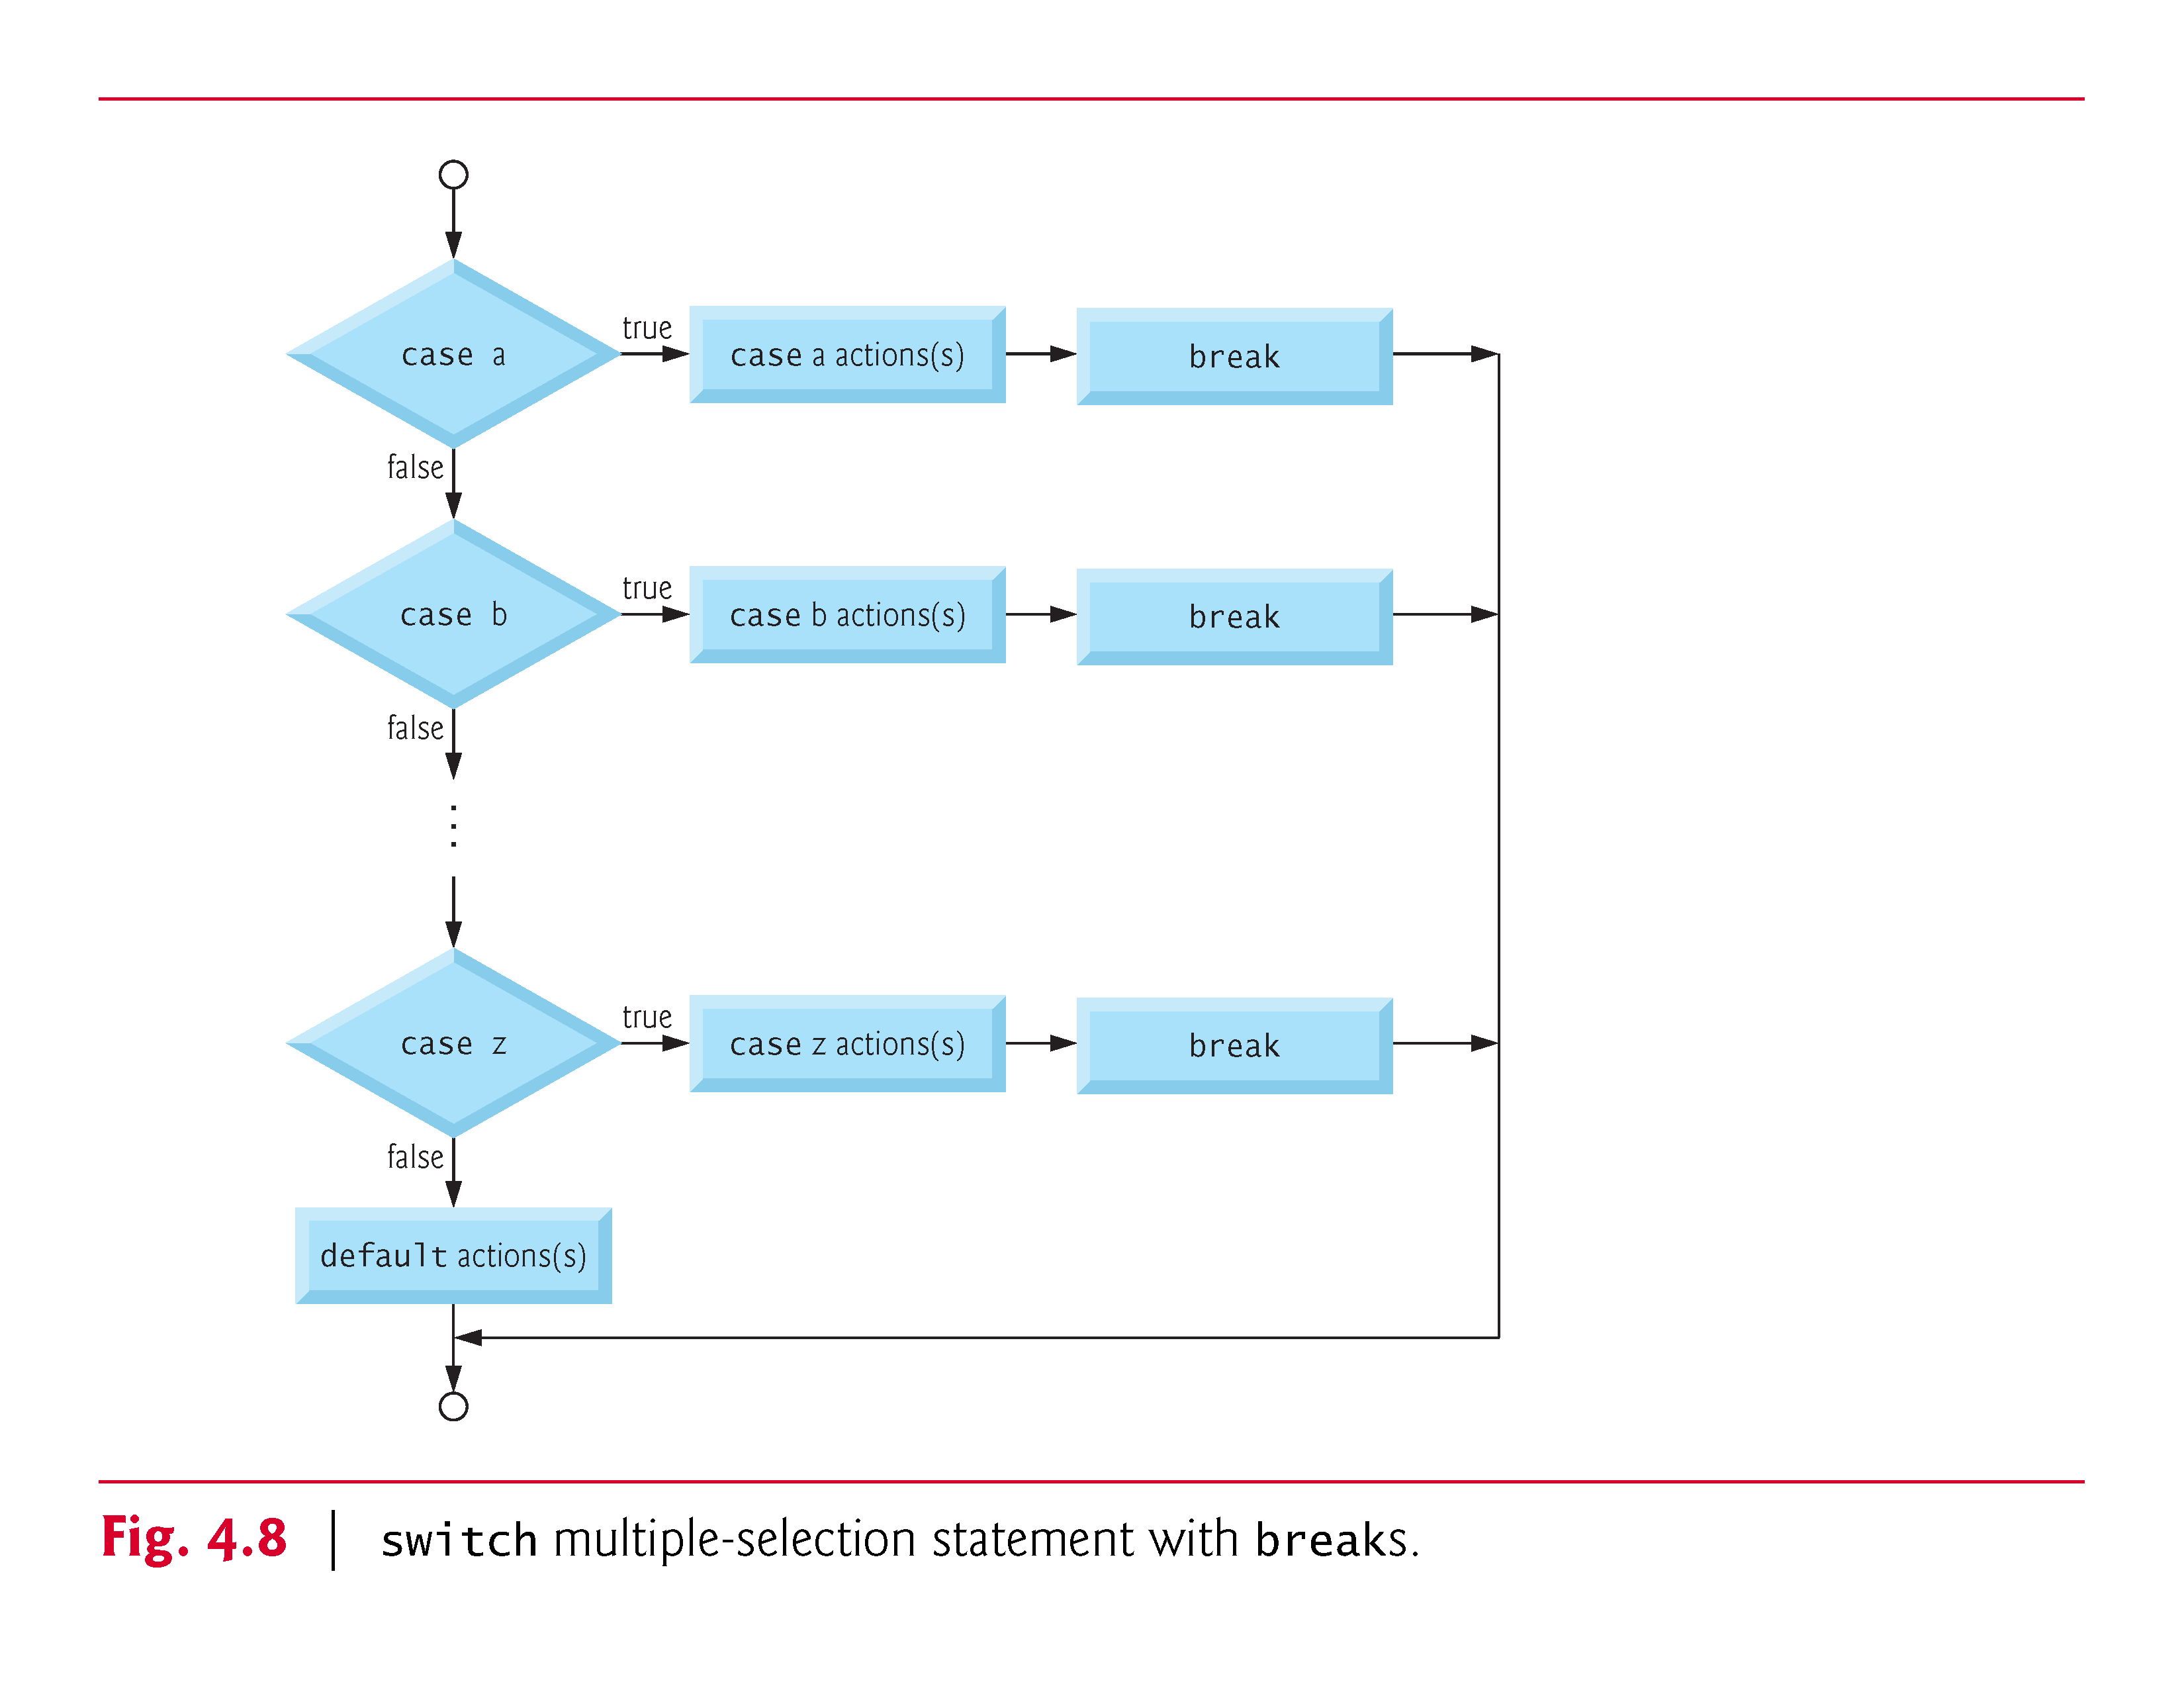
\includegraphics[scale=0.35]{switchflowchart.png}
\end{frame}

\begin{frame}[fragile=singleslide]{Let's \texttt{switch} to an example! }
\begin{lstlisting}[style=C]
#include<stdio.h>

int main (void) {
	char grade;
	printf("Enter your grade: \n");
	scanf("%c", &grade);
	switch (grade) {
		case 'A':
			printf("Amazing! A smart person! ");
		case 'B':
			printf("You have met expectations.\n");
			break;
		case 'C':
			printf("You need to study harder! ");
		case 'D':
			printf("At least you passed!\n");
			break;
\end{lstlisting}
\end{frame}

\begin{frame}[fragile=singleslide]{Let's \texttt{switch} to an example! }
\begin{lstlisting}[style=C]
		case 'F':
			printf("Well, they're always hiring in the army.\n")
			break;
		default :
			printf("That's not even a proper grade!\n");
			break;
	}
}
\end{lstlisting}
\hrule
\vspace{1em}
\emph{Cue Demonstration}
\end{frame}

\section[Loops]{Iterative Structures}
\begin{frame}{Going Loopy}
In C, there are three types of loops: 
\begin{itemize}
\item \texttt{while}
\item \texttt{do while}
\item \texttt{for}
\end{itemize}
There are also two control statements for use in loops:
\begin{itemize}
\item \texttt{break;}
\item \texttt{continue;}
\end{itemize}
\end{frame}

\begin{frame}[fragile=singleslide]{\texttt{do while} I think of Another Pun}
\begin{itemize}
\item \texttt{while} loops in C work the same way as in Python 
\item \texttt{do while} loops are a slight variation:
\begin{lstlisting}[style=C]
	// <Initializing Statement>
	do {
		// <Body Statements>
		// <Update Statement>
	} while (/*<Condition>*/); 
\end{lstlisting}
\item \texttt{while} loops test their conditions \emph{before} each loop iteration.
\item \texttt{do while} loops test their conditions \emph {after} each loop iteration.
\item This means that a \texttt{do while} loop must execute \emph{at least one} loop iteration.  
\item Aside from that, there is no semantic difference between \texttt{while} and \texttt{do while} loops.  
\end{itemize}
\end{frame}

\begin{frame}[fragile=singleslide]{\texttt{for}midable Coding}
\begin{itemize}
\item In Python, a for loop is used to iterate over the elements of a data structure (lists, dictionaries, etc.)
\item In C, for loops are just syntactic sugar for a while loop.
\end{itemize}
\begin{lstlisting}[style = C]
// Countdown from 10 using a while loop
	int i = 10;
	while (i >= 0) {
		printf("%d...\n",i);
		i --;
	}	
// Countdown from 10 using a for loop
	for (int i = 10; i >= 0; i--) {
		printf("%d...\n",i);
	}
\end{lstlisting}
\end{frame}

\begin{frame}{\texttt{continue}... and \texttt{break} for lunch!}
Two statements may be used to control loop execution outside of the loop's main conditional.
\begin{itemize}
\item \texttt{break} - exits the loop
\begin{itemize}
	\item When the program pointer hits a \texttt{break} statement, the loop it's in is immediately terminated, as if it's conditional test had returned false.  
	\item \texttt{break} can be very useful for programs with complex logic
	\item The truth literal can even be used as the loop conditional if the program breaks correctly.
	\item \texttt{break} is also used in \texttt{switch case} blocks.
\end{itemize}
\item \texttt{continue} - starts next iteration
\begin{itemize}
\item Jumps immediately to the next iteration of a loop.
\item The applications are not as numerous, most people use if-branching to not execute the rest of the code inside a loop, but \texttt{continue} can reduce the indentation level of your code.  
\end{itemize}
\end{itemize}

\end{frame}

\begin{frame}{The last slide comic...}
\center
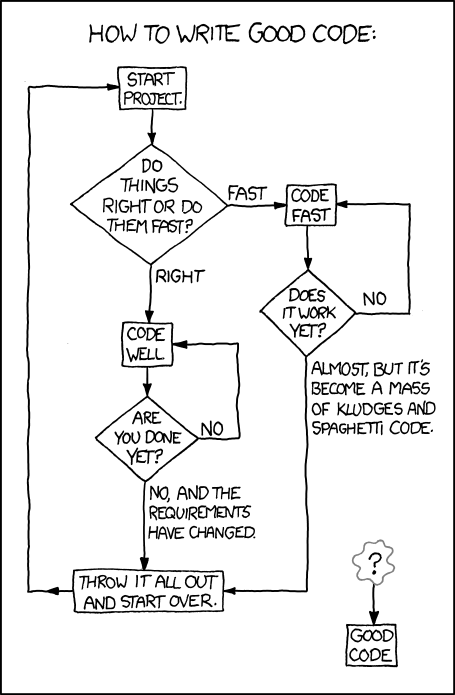
\includegraphics[scale=0.3]{good_code.png}
\end{frame}

\end{document}
